\paragraph{}
La problématique principale du projet fut de concevoir une architecture logicielle qui reflète la fonctionnement de console mais qui puisse aussi être modulaire. En effet, les composants de la NES communiquent les un avec les autres à travers l'espace d'adressage du processeur 6502, la cartouche de jeu y compris. Avec le format cartouche, il est tout à fait possible de moduler le circuit électronique de la cartouche pour augmenter la capacité de stockage du programme ou sauvegarder des parties. Nous constatons alors que l'espace d'adressage varie d'un type de cartouche (ou \emph{mapper} dans le langage technique de la console) à un autre.

\paragraph{}
\begin{wrapfigure}{r}{0.45\textwidth}
  \centering
  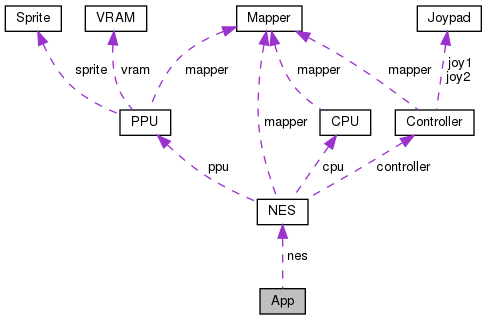
\includegraphics[width=1\linewidth]{images/struct_app}
  \caption{Structure de l'application}
  \label{fig:struct_app}
\end{wrapfigure}
Nous avons donc développé notre émulateur sur un modèle orienté objet : chaque structure est accompagné de fonctions constructrice, destructrice et fonctionnelles. Ce modèle nous permet de gagner en modularité : lors d'un chargement de ROM, venir charger l'espace mémoire correspondant au mapper et ce de manière transparente pour le reste du système. Vous retrouvez sur la figure \ref{fig:struct_app} l'architecture de l'émulateur du point de vue des structures.
